Spectroscopy measures absorption and emission of light and other radiation by matter \cite{atascientificUnderstandingSpectrometrySpectroscopy2020}. The energy, wavelength, or frequency of photons that pass through a sample is detected. In the particular case of THz-TDS, matter is probed with very short THz pulses. The pulse usually has a duration of a few picoseconds \cite{neuTutorialIntroductionTerahertz2018}. The THz time domain signal is a measure of the transient electrical field. This is a major advantage of THz-TDS because intensity and phase of the electrical field are measured simultaneously \cite{zhaoPrincipleTerahertzTimeDomain2023}.

A conventional THz-TDS system consists of a femtosecond laser, a THz source, mirrors for beam steering, delay stages, optical beam splitters, focusing and collimating optics, and a THz detector. A more detailed description of the components in a THz-TDS system is given in Section \ref{setup}.

The basic working principle of THz-TDS is described in the following, mainly as a review of \cite{neuTutorialIntroductionTerahertz2018,PrinciplesTerahertzScience2009,nandiErAsInAlGaAsPhotoconductors2021}. 
In a pulsed THz-TDS system, an ultrafast laser is used to drive both the THz detector and source. As the electrical field of the THz signal usually has a time duration of a few picoseconds, optical detection techniques with sub-picosecond resolution are needed. The laser's pulse duration lies in the $\sim$ \num{100} \si{\femto\s} range. This ultrashort near infrared (NIR) optical pulse is beamsplit along two paths to generate and detect the time dependent THz field. One of the beams goes through a translational stage to provide a relative time delay. The time delay ensures that we can measure the amplitude of the pulse's electrical field at the detector at multiple points in time. The temporal delay is achieved by increasing the path length of the beam. The travel time of a laser pulse is $t = s/c$, where $s$ is the path length and $c$ is the speed of light. The other beam is used as an optical pump signal, illuminating the THz emitter to generate the THz signal. The signal is focused onto a THz detector. Here, the electrical field of the THz signal is measured by using the delayed beam as a probing pulse. The THz field is measured in the time-domain. THz-TDS makes use of the convolution of the short probing pulse with the longer THz signal. The instantaneous signal at the detector can be described as 

\begin{equation}
	S(t) \propto I_{opt}(t)\cdot E_{THz}(t),
\end{equation}

with $I_{opt}(t)$ being the optical intensity of the probing pulse and $E_{THz}(t)$ being the THz field at the detector interface. This signal must be detected with subpicosecond resolution. All existing detectors are too slow, so the convolution of the two pulses is measured instead: 

\begin{equation}
	S(t) \propto I_{opt}(t) \ast E_{THz}(t).
\end{equation}

Note that ($\ast$) denotes the convolution operator here. The duration of the optical probing pulse is significantly shorter than the duration of the THz signal. We can approximate it as an ideal pulse, hence the delta-function $\delta(t)$, yielding

\begin{equation}
	S(t) \propto I_{opt}(t) \ast E_{THz}(t) \approx \delta(t) \ast E_{THz}(t) = E_{THz(t)}.
\end{equation}

Because of the convolution, the THz detector is only sensitive when both signals arrive at the same time. The THz-field is only measured at one specific point in time. By varying the path length $s$ of the probing pulse, we can scan through the complete pulse in the time-domain by taking a set of time-discrete measurements (see Figure \ref{fig:convo}). The probing pulse being approximated as the delta-function allows us to measure the amplitude and phase of the THz signal as a function of time. With knowledge about the amplitude and the phase, not only the absorption but also the dispersion of the sample can be obtained by analyzing the Fourier transforms of the waveforms. 

\begin{figure}[!]
  \centering
  % \begin{minipage}{0.5\textwidth}
    \centering
    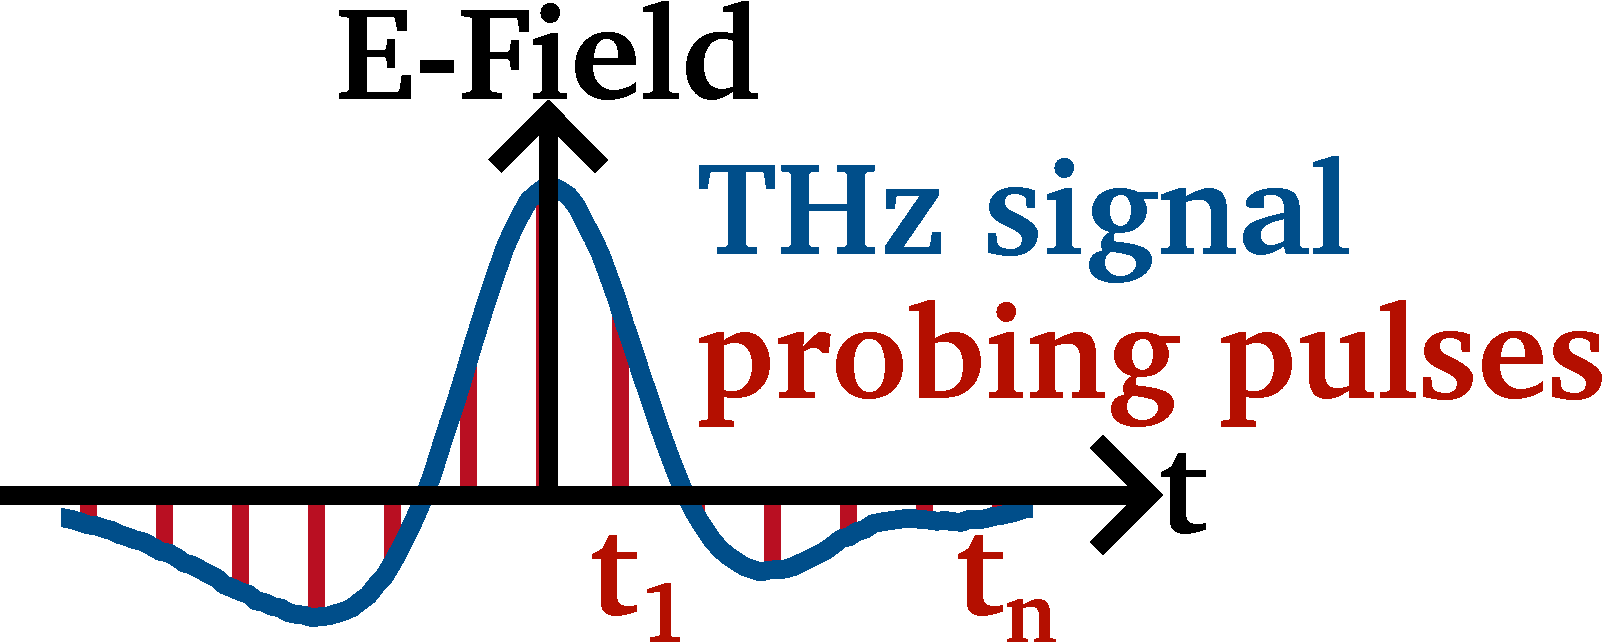
\includegraphics[width=0.4\linewidth]{figures/theory/TDS_basics.pdf}
    \caption{Schematic depiction of the sampling of a THz pulse via convolution of two signals. The probing pulse measures the electric field of the incident THz radiation at discrete points in time. By varying the relative path length difference of the probing signal and the THz signal, the probing pulses scan through the complete THz wave in the time-domain.} 
    \label{fig:convo}
  % \end{minipage}
\end{figure}